In this appendix we compute the Riemannian gradients and hessian vector products for the cost functions \eqref{eq:YB_move_disent_cost_function_truncation_error} and \eqref{eq:renyi_entropy}. For this it is first necessary to derive the derivative of the complex-valued singular value decomposition (SVD), which we show in Section \ref{sec:derivative_of_SVD}. The derivation is similar to \cite{cite:differentiating_the_svd}. We then proceed by deriving the gradients in section \ref{sec:renyi_trunc_gradients} and the hessian vector products in section \ref{sec:renyi_trunc_hvps}.
\section{Derivative of the SVD}
\label{sec:derivative_of_SVD}
Let $A\in\mathbb{C}^{m\times n}$ of rank $k \le \min(m,n)$. The SVD of $A$ is defined as $A = USV^\dagger$, with $U\in\mathbb{C}^{m\times k}$, $S\in\mathbb{R}^{k\times k}$ diagonal, $V\in\mathbb{C}^{n\times k}$ and
\begin{equation}
	\label{eq:derivative_svd_eq_1}
	 U^\dagger U = \quad V^\dagger V = \id_k.
\end{equation}
In this definition we already truncated singular values $s_j = 0$, such that $S$ has only non-zero entries on the diagonal. Let $\text{d}A\in\mathbb{C}^{m\times n}$ be an infinitesimal change of $A$. We are interested in the infinitesimal changes $\text{d}U$, $\text{d}S$ and $\text{d}V$ that are obtained when performing the SVD $(A+\text{dA}) = (U + \text{d}U)(S + \text{d}S)(V + \text{d}V)^\dagger$. Up to first order we obtain
\begin{equation}
	\label{eq:derivative_svd_eq_2}
	\text{d}A = \text{d}USV^\dagger + U\text{d}SV^\dagger + US\text{d}V^\dagger.
\end{equation}
Differentiating Equation \eqref{eq:derivative_svd_eq_1} yields $\text{d}U^\dagger U + U^\dagger\text{d}U = 0$ and $\text{d}V^\dagger V + V^\dagger\text{d}V = 0$. It follows that $\text{d}\Omega_U \coloneqq U^\dagger\text{d}U$ and $\text{d}\Omega_V \coloneqq V^\dagger\text{d}V$ are $k\times k$ anti-hermitean matrices. One can then always find hermitean matrices $U_\perp\in\mathbb{C}^{m\times(m-k)}$ and $V_\perp\in\mathbb{C}^{n\times(n-k)}$ such that $\left[U\,U_\perp\right]$ and $\left[V V_\perp\right]$ are unitary and it holds $U^\dagger U_\perp = 0$ and $V^\dagger V_\perp = 0$. This procedure is called unitary completion and can for example be computed by using the Gram-Schmidt algorithm. The notation $\left[U\,U_\perp\right]$ means stacking the columns of $U$ and $U_\perp$ to form a $m\times m$ matrix. We may now expand $\text{d}U$ as
\begin{equation}
	\label{eq:dOmega_U_definition}
	\text{d}U = U\text{d}\Omega_U + U_\perp\text{d}K_U
\end{equation}
and $\text{d}V$ as
\begin{equation}
	\label{eq:dOmega_V_definition}
	\text{d}V = V\text{d}\Omega_V + V_\perp\text{d}K_V,
\end{equation}
with $\text{d}K_U\in\mathbb{C}^{(m-k)\times k}$ and $\text{d}K_V\in\mathbb{C}^{(n-k)\times k}$ to be determined. We proceed by left-multiplying \eqref{eq:derivative_svd_eq_2} by $U^\dagger$ and right-multiplying by $V$ to obtain
\begin{equation}
	\label{eq:svd_derivative_P_definition}
	\begin{split}
		\text{d}P \coloneqq U^\dagger\text{d}AV &= U^\dagger\text{d}US + \text{d}S + S\text{d}V^\dagger V \\
		&= \text{d}\Omega_U S + \text{d}S + S\text{d}\Omega_V^\dagger.
	\end{split}
\end{equation}
Since $\text{d}\Omega_U$ and $\text{d}\Omega_V$ are anti-hermitean, there diagonal elements are purely imaginary. However, $\text{d}S$ is a diagonal matrix with purely real entries. Thus it is immediately clear that
\begin{equation}
	\label{eq:dS_final}
	\text{d}S = \id_k \circ \Re\left[\text{d}P\right],
\end{equation}
with the \textit{Hadamard product} $(A\circ B)_{i,j} = A_{i,j}\cdot B_{i,j}$. It further follows
\begin{equation}
	\label{eq:derivative_svd_eq_3}
	\text{d}\Omega_US - S\text{d}\Omega_V = \id_k\circ i\Im\left[\text{d}P\right] + \bar{\id}_k\circ\text{d}P.
\end{equation}
Here, the notation $\bar{\id}_k$ means a $k\times k$ matrix with zeros on the diagonal and ones everywhere else. Taking the complex conjugate of \eqref{eq:derivative_svd_eq_3} yields \begin{equation}
	\label{eq:derivative_svd_eq_4}
	-S\text{d}\Omega_U + \text{d}\Omega_V S = -\id_k\circ i\Im\left[\text{d}P\right] + \bar{\id}_k\circ\text{d}P^\dagger.
\end{equation}
To proceed we right-multiply \eqref{eq:derivative_svd_eq_3} by $S$, left-multiply \eqref{eq:derivative_svd_eq_4} by $S$ and add the two equations together, yielding
\begin{equation}
	\label{eq:equation_for_solving_dOmega_U}
	\text{d}\Omega_U S^2 - S^2 \text{d}\Omega_U = \bar{\id}_k\circ S\text{d}P + \bar{\id}_k\circ \text{d}P^\dagger S = \bar{\id}_k\circ\left[\text{d}PS+S\text{d}P^\dagger\right],
\end{equation}
where we used the fact that $D(A\circ B) = DA\circ B = A\circ DB$ and $(A\circ B)D = AD\circ B = A\circ BD$ for diagonal matrices $D$. We now want to solve Equation \eqref{eq:equation_for_solving_dOmega_U} for $\text{d}\Omega_U$. The solution is given by
\begin{equation}
	\label{eq:derivative_svd_eq_5}
	\text{d}\Omega_U = F\circ\left[\text{d}PS+S\text{d}P^\dagger\right]
\end{equation}
with 
\begin{equation}
	\label{eq:svd_derivative_F_definition}
	F_{i,j} \coloneqq \begin{cases}
		\frac{1}{d_j^2-d_i^2} &i \neq j\\
		0 &i = j
	\end{cases},
\end{equation}
which can be easily checked by inserting. We can obtain a similar equation for $\text{d}\Omega_V$ by left-multiplying \eqref{eq:derivative_svd_eq_3} by $S$ and right-multiplying \eqref{eq:derivative_svd_eq_4} by $S$ before adding the two equations. The resulting equation is solved by
\begin{equation}
	\label{eq:derivative_svd_eq_6}
	\text{d}\Omega_V = F\circ\left[S\text{d}P+\text{d}P^\dagger S\right].
\end{equation}
Equations \eqref{eq:derivative_svd_eq_5} and \eqref{eq:derivative_svd_eq_6} do not fix the diagonals of $\text{d}\Omega_U$ and $\text{d}\Omega_V$. We can determine these remaining free parameters by looking at the diagonal elements of equation \eqref{eq:derivative_svd_eq_3}:
\begin{equation}
	\begin{split}
		&\id_k\circ\left[\text{d}\Omega_US-S\text{d}\Omega_V\right] = \id\circ i\Im\left[\text{d}P\right] \\
		\Rightarrow \quad &\id_k\circ\left[\text{d}\Omega_U-\text{d}\Omega_V\right] = \id_k\circ i\Im\left[\text{d}P\right]S^{-1}.
	\end{split}
\end{equation}
We can solve this equation by setting
\begin{equation}
	\begin{split}
		\text{d}\Omega_U &= F\circ\left[\text{d}PS + S\text{d}P^\dagger\right] + \id_k\circ\text{d}D,\\
		\text{d}\Omega_V &= F\circ\left[S\text{d}P + \text{d}P^\dagger S\right] - \id_k\circ\text{d}D,
	\end{split}
\end{equation}
with
\begin{equation}
	\text{d}D \coloneqq \frac{i}{2}\Im\left[\text{d}P\right]S^{-1}.
\end{equation}
It remains to find $\text{d}K_U$ and $\text{d}K_V$. We can compute $\text{d}K_U$ by left-multiplying \eqref{eq:derivative_svd_eq_2} by $U_\perp^\dagger$ and right-multiplying by $VS^{-1}$, yielding
\begin{equation}
	\label{eq:derivative_svd_eq_7}
	\text{d}K_U = U_\perp^\dagger \text{d}AVS^{-1}.
\end{equation}
Similarly, we can left-multiply \eqref{eq:derivative_svd_eq_2}$^\dagger$ by $V_\perp^\dagger$ and right-multiplying by $US^{-1}$ to obtain
\begin{equation}
	\label{eq:derivative_svd_eq_8}
	\text{d}K_V = V_\perp^\dagger\text{d}A^\dagger US^-1.
\end{equation}
Putting everything together, we obtain
\begin{equation}
	\label{eq:final_solution_svd_derivative}
	\begin{split}
		\text{d}U &= U\left(F\circ\left[\text{d}PS+S\text{d}P^\dagger\right] + \id_k\circ\text{d}D\right) + \left(\id_m-UU^\dagger\right)\text{d}AVS^{-1}. \\
		\text{dS} &= \id_k\circ\Re\left[\text{d}P\right]. \\
		\text{d}V &= V\left(F\circ\left[D\text{d}P+\text{d}P^\dagger S\right] - \id_k\circ\text{d}D\right) + \left(\id_n-UU^\dagger\right)\text{d}AUS^{-1},
	\end{split}
\end{equation}
with $\text{d}P$ defined as \eqref{eq:svd_derivative_P_definition} and $F$ defined as \eqref{eq:svd_derivative_F_definition}. To arrive at the final expressions for $\text{d}U$ and $\text{dV}$ we used the fact that $M_U \coloneqq \left[U\,U_\perp\right]$ and $M_V \coloneqq \left[V V_\perp\right]$ are unitary and thus $M_UM_U^\dagger = UU^\dagger + U_\perp U_\perp^\dagger = \id_m$ and similarly $VV^\dagger + V_\perp V_\perp^\dagger = \id_n$ to eliminate $U_\perp U_\perp^\dagger$ and $V_\perp V_\perp^\dagger$. \par
There is one small subtlety left to discuss. The SVD is not unique, but has a gauge degree of freedom: A diagonal matrix of complex phases $\Lambda_{j,j} = e^{i\theta_j}$ can be inserted as $A = USV^\dagger = U^\prime S V^{\prime\dagger} = (U\Lambda)S(V\Lambda)^\dagger$. This means that the exact values of $\text{d}U$ and $\text{d}V$ are ill-defined and it is only possible to compute derivatives of functions that are gauge-invariant, i.e. functions where $\Lambda$ is cancelled with its adjoint.
%
%
\section{Gradients}
%
%
\label{sec:renyi_trunc_gradients}
We now compute Riemannian gradients for the two cost functions discussed in Section \ref{sec:YB_move_svd_disentangle}, namely the truncation error
\begin{equation}
	\label{eq:appendix_trunc_error_cost_function}
	f_\text{trunc}\left(U,\theta\right) = \sqrt{\sum_{\mu = \chi+1}^{\chi D^2}S_\mu^2} = \sqrt{1 - \sum_{\mu = 1}^{\chi}S_\mu^2}
\end{equation}
and the Rényi-entropy
\begin{equation}
	\label{eq:appendix_renyi_cost_function}
	f_\text{Rényi}\left(U,\theta,\alpha\right) = \frac{1}{1-\alpha}\log\Tr\left(\rho^\alpha\right) = \frac{1}{1-\alpha}\log\left(\sum_{\mu=1}^{\chi D^2}S_\mu^{2\alpha}\right).
\end{equation}
The singular values stem from the SVD $U\theta$ = $XSY$ as shown in figure \figref{fig:disentangling_theta_definition}. We first compute the derivative of a single singular value $S_\mu$ with respect to $U$. Using the product rule for matrices \cite{cite:the_matrix_cook_book} and the derivative of the SVD \eqref{eq:final_solution_svd_derivative}, we obtain
\begin{center}
	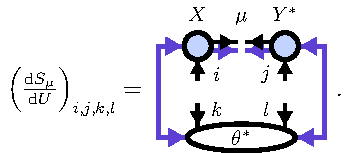
\includegraphics[scale=1]{figures/tikz/gradient_and_hvp/derivative_of_s_mu/derivative_of_s_mu.pdf}
\end{center}
We can then use this result to compute the derivative of the truncation error as
\begin{equation}
	\frac{\text{d}}{\text{d}U}f_\text{trunc}(U,\theta) = -\frac{1}{f_\text{trunc}(U,\theta)}\sum_\mu S_\mu \frac{\text{d}S_\mu}{\text{d}U}
\end{equation}
and the derivative of the Rényi-entropy as
\begin{equation}
	\frac{\text{d}}{\text{d}U}f_\text{Rényi}(U,\theta,\alpha) = \frac{2\alpha}{1-\alpha}\frac{1}{\sum_\mu S_\mu^{2\alpha}} \sum_\mu S_\mu^{2\alpha-1}\frac{\text{d}S_\mu}{\text{d}U}.
\end{equation}
As a last step, the derivatives must be projected back to the tangent space of $U$, see Equation \eqref{eq:riemannian_optimization_gradient_of_cost_function}. We obtain
\begin{equation}
	\left(\nabla f_\text{trunc}\left(U,\theta\right)\right)_{i,j,k,l} = \frac{1}{2f_\text{trunc}\left(U,\theta\right)}\xi^\text{trunc}_{i,j,k,l}
\end{equation}
and
\begin{equation}
	\left(\nabla f_\text{Rényi}\left(U,\theta,\alpha\right)\right)_{i,j,k,l} = \frac{\alpha}{1-\alpha}\frac{1}{\sum_\mu S_\mu^{2\alpha}}\xi^\text{Rényi}_{i,j,k,l}
\end{equation}
respectively, with
\begin{center}
	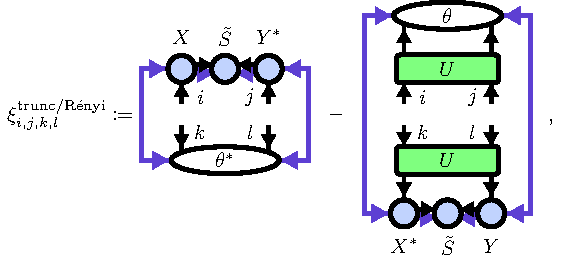
\includegraphics[scale=1]{figures/tikz/gradient_and_hvp/xi_definition/xi_definition.pdf}
\end{center}
where $\tilde{S} = S$ for $\xi^\text{trunc}$ and $\tilde{S} = S^{2\alpha-1}$ for $\xi^\text{Rényi}$.
%
%
\section{Hessian vector products}
\label{sec:renyi_trunc_hvps}
%
%
In this section we compute the hessian vector product of $\nabla f$ and $\Delta U$. We start by first calculating the directional derivative of the gradient
\begin{equation}
	\text{D}\left(\nabla f\right)\left[U\right],
\end{equation}
which we subsequently need to project to the tangent space of $U$. For matrix multiplication it holds\cite{cite:the_matrix_cook_book}
\begin{equation}
	\text{D}\left(AB\right)\left[\Delta A\right] = \Delta AB.
\end{equation}
Directional derivatives of $X$, $U$ and $Y$ can be obtained with equation \eqref{eq:final_solution_svd_derivative} by setting $\text{d}A = \Delta U\theta$. The final result are the directional derivatives
\begin{multline}
	\big((\text{D}(\nabla f_\text{trunc})[\Delta U]\big)_{i,j,k,l} = \\
	-\frac{1}{2f_\text{trunc}(U, \theta)} \cdot \left\{\frac{1}{f_\text{trunc}(U,\theta)^2}\sum_{\mu=1}^{\chi}S_\mu\big(\text{D}S_\mu[\Delta U]\big)\xi_{i,j,k,l} + G^\text{trunc}_{i,j,k,l}\right\}
\end{multline}
and
\begin{multline}	
	\big(\text{D}(\nabla f_\text{Rényi})[\Delta U]\big)_{i,j,k,l} = \\
	\frac{\alpha}{1-\alpha} \left\{\frac{2\alpha}{\left(\sum_\mu S_\mu^{2\alpha}\right)^2}\sum_\mu S_\mu^{2\alpha-1}\text{d}S_\mu\xi_{i,j,k,l} + \frac{1}{\sum_\mu S_\mu^{2\alpha}}G^\text{Renyi}_{i,j,k,l}\right\}
\end{multline}
with the definition of $G^\text{trunc}$ and $G^\text{Rényi}$ given in tensor diagram notation in Figure \figref{fig:G_definition}. Finally, The derivatives must be projected to the tangent space of $U$, see Equation \eqref{eq:riemannian_optimization_gradient_of_cost_function}.
\begin{figure}
	\centering
	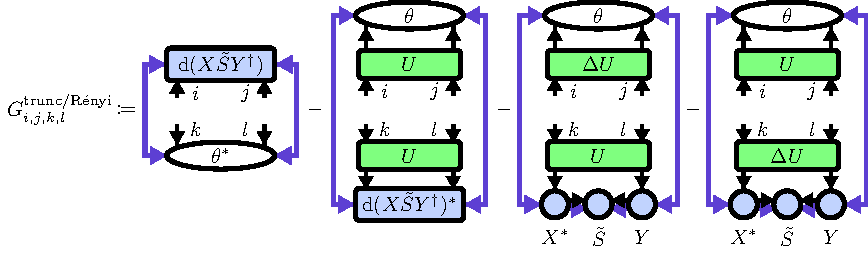
\includegraphics[scale=0.9]{figures/tikz/gradient_and_hvp/G_definition/G_definition.pdf}
	\caption{In this figure we give the definition for $G^\text{trunc}$ and $G^\text{Rényi}$ in tensor diagram notation. For $G^\text{trunc}$ we set  $\tilde{S} = S$ and for $G^\text{Rényi}$ we set  $\tilde{S} = S^{2\alpha-1}$. The definition of $\text{d}(X\tilde{S}Y)$ is given in figure \protect\figref{fig:dXSY_definition}}
	\label{fig:G_definition}
\end{figure}
\begin{figure}
	\centering
	\subcaptionbox{\label{fig:dXSY_definition_trunc}}
	{%
		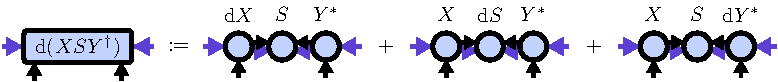
\includegraphics[scale=1]{figures/tikz/gradient_and_hvp/dXSY_definition/dXSY_definition_a.pdf}
	}
	\par\bigskip
	\subcaptionbox{\label{fig:dXSY_definition_rewnyi}}
	{%
		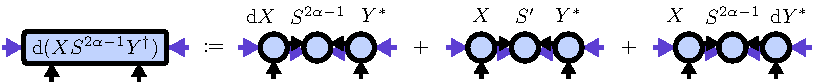
\includegraphics[scale=1]{figures/tikz/gradient_and_hvp/dXSY_definition/dXSY_definition_b.pdf}
	}
	\caption{The definitions for (a) $\text{d}(XSY^\dagger)$ and (b) $\text{d}(XS^{2\alpha-1}Y^\dagger)$ are given in tensor diagram notation. In (b), we use $S_\mu^\prime \coloneqq (2\alpha-1)S_\mu^{2\alpha-2}\text{d}S_\mu$.}
	\label{fig:dXSY_definition}
\end{figure}